\chapter{Tworzenie polskich zbiorów}
W ostatnim czasie w szczególności nacisk zostaje przenoszony z modeli na odpowiednie przygotowanie i jakość zbiorów danych. Przykładem tego jest wydany w ostatnim czasie artykuł \bibtitle{Textbooks are all you need} \cite{Gunasekar2023}, który demonstruję jak dużą poprawę można uzyskać bez powiększania i komplikowania wykorzystywanego modelu, lecz poprzez stworzenie wysokiej jakości zbioru danych.

Jako, że dla zadania \code{Text-to-SQL} na moment pisania niniejszej pracy nie istnieją żadne zbiory danych w języku polskim, a także ze względu na duże ich znaczenie, wiele uwagi zostało poświęcone tej kwestii. 

Na początku bieżącego rozdziału omówione zostaną przyjęte założenia dotyczące tworzenia polskich zbiorów, a następnie przedyskutowane dokładnie dwa kluczowe dla tego procesu elementy: dynamiczne generowanie oraz sposób dokonywania tłumaczenia. Ostatecznie nastąpi analiza i podsumowanie stworzonych zbiorów.

\section{Przyjęte założenia}
Po przeanalizowaniu różnic pomiędzy istniejącymi tłumaczeniami zbioru \code{Spider} określone zostały założenia przyjęte na potrzebę stworzenia zbiorów polskich.

% To fix:
Podczas tłumaczenia zbiorów przyjęto dwa podstawowe założenia. Pierwszym jest wykorzystanie tłumaczenia maszynowego, zamiast manualnego. Drugi stanowi dynamiczne generowanie finalnych zbiorów zamiast jednorazowego tłumaczenia wszystkich przykładów i udostępnienia jedynie zmodyfikowanej ich wersji. Oba założenia zostaną rozwinięte, uzasadnione i dokładnie przedyskutowane w poniższych dwóch sekcjach.

\subsubsection{Tłumaczenie maszynowe}
Pomimo wskazanej w sekcji \ref{text:translation-method} dominacji tłumaczenia manualnego nad maszynowym postanowiono wykorzystać to ostatnie. Przyczyn takiej decyzji jest kilka. Przede wszystkim w realizację tłumaczenia aktywnie zaangażowana jest jedynie jedna osoba, w odróżnieniu do wcześniejszych prac, w których w tym procesie uczestniczyło ich kilka, a w przypadku rosyjskiego zbioru nawet profesjonalny tłumacz. Drugą przesłanką jest ograniczony czas, ze względu na pracę magisterką w ramach której niniejszy temat jest realizowany. Ostatecznie jest to zadanie żmudne, a zbiór maszynowy, pomimo niższej jakości, także pozwoli, a nawet da więcej czasu, na wykonanie eksperymentów.

\subsubsection{Dynamiczne generowanie}
Wszystkie dotychczasowe tłumaczenia zbioru Spider sprowadzają się jedynie do udostępnienia zmodyfikowanej wersji zbioru, bez żadnych dodatkowych skryptów. Wydaje się to wystarczające i dla większości zastosowań w rzeczywistości jest. Taki zbiór stanowi bardzo dobry benchmark służący do porównywania różnych algorytmów, ponieważ nie ma żadnych niedomówień w kwestii jego zawartości.

Podjęcie innowacyjnego podejścia polegającego na generowaniu finalnego zbioru z odpowiednio przygotowanych elementów składowych ma jednak szereg zalet. Jedną z nich jest brak konieczności podejmowania kategorycznej decyzji odnośnie wyboru języka schematu baz danych - można wygenerować różne warianty podając różne parametry do polecenia generującego. Podobnie nie trzeba decydować, czy wartości w zapytaniach SQL mają być tłumaczone. Jest to więc podejście bardzo elastyczne i otwierające drogę do przeprowadzania różnorodnych eksperymentów.

\subsubsection{Oryginalna zawartość baz danych}
Zawartość baz danych postanowiono pozostawić bez tłumaczenia. Jest to podejście pokrywające się z większością istniejących tłumaczeń zbioru \code{Spider}. Powodem do tego jest duża ilość znajdujących się w bazach informacji, których tłumaczenie skutkowałoby naliczeniem dodatkowych kosztów. Oferowane przez użyty tłumacz DeepL darmowe limity tłumaczeń zostały całkowicie wykorzystane na przetłumaczenie pytań oraz wartości w zapytaniach SQL, co było bezpośrednią przyczyną podjęcia powyższej decyzji.

\subsubsection{Tłumaczenie dodatkowych zbiorów}
Kolejnym z powziętych założeń zostało, oprócz przetłumaczenia zbioru \code{Spider}, również przetłumaczenie kilku dodatkowych zbiorów (przedstawionych wcześniej w sekcji \ref{text:related-datasets}) wykorzystujących te same bazy danych. Jest to ułatwione, ponieważ dzięki wspólnym bazą danych nie jest konieczne ponowne dokonywanie tłumaczenia ich schematu. Zastosowane podejście z dynamicznym generowaniem jeszcze bardziej uprasza proces tłumaczenia dodatkowych zbiorów, więc postanowiono to wykorzystać. Nie znaleziono żadnych informacji na temat tego typu wcześniejszych badań i być może jest to pierwsza próba tłumaczenia tych zbiorów.

\section{Dynamiczne generowanie}
Dynamiczne generowanie różnych wariantów zbioru jest ważnym elementem niniejszej pracy i w znaczny sposób odróżnia ją od wcześniejszych podejść. W związku z tym zostanie ono w tej części dokładnie opisane.

Implementacja tej strategii sprowadza się do stworzenia skryptu pozwalającego na wygenerowanie zbioru o żądanych parametrach. Wśród nich możliwe jest określenie języka pytań, języka wartości w zapytaniach i wariantu tłumaczenia schematu bazy danych.

Na początku przedstawione zostaną nowo wprowadzone formaty plików, które stworzony skrypt wykorzystuję do generowania wariantów zbioru.


\subsection{Wprowadzone formaty plików}
W celu umożliwienia generowania różnych wariantów zbioru konieczne było zmodyfikowanie istniejących plików z próbkami poprzez dodanie przetłumaczonych wersji pytań i zapytań SQL oraz opracowany został kompletnie nowy format plików zawierających informację na temat tego jak mają być tłumaczone nazwy tabel i kolumn.

\subsubsection{Format próbek}
Na listingu \ref{lst:new-sample} przedstawiony został format próbek wykorzystany w procesie syntezy zbioru. Porównując ten plik z oryginalnym formatem ze zbioru Spider (przedstawionym wcześniej na listingu \ref{lst:spider-sample}) widać, że zostały dodane polskie odpowiedniki pytań naturalnych oraz zapytań SQL. Nic nie stoi na przeszkodzie dodaniu kolejnego języka, na przykład istniejących już tłumaczeń chińskich lub rosyjskich. W zależności od parametrów podanych do skryptu generującego wybierany jest odpowiedni język. 

\begin{minipage}{\linewidth}
\lstinputlisting[
caption=Fragment pliku \code{tables.json} opisujący schemat pojedynczej bazy danych, label={lst:new-sample}, language=json
]{listings/new_sample.json}
\end{minipage}

Dodatkowo format ten został odchudzony o wszystkie redundantne atrybuty, takie jak tokeny pytania, tokeny zapytania SQL i sparsowane zapytania SQL. Komplikowały one proces tłumaczenia, bo wymagały wprowadzania tych samych zmian w kilku miejscach i narażały zbiór na niespójność. Z tego powodu postanowiono je usunąć z plików zbioru i dodawać dynamicznie podczas jego finalnego generowania.

\subsubsection{Format mapowania nazwy schematu}
Aby umożliwić dokonywanie różnych tłumaczeń schematu baz danych opracowany został format pliku przedstawiony na listingu \ref{lst:new-trans}. Zawiera on informacje pozwalające dokonać mapowania oryginalnych nazw na dowolne inne. Jest to plik json o kilku stopniach zagnieżdżenia. Na najwyższym poziomie jest słownikiem, który dla każdej nazwy bazy zawiera listę tabel, a każda tabela listę kolumn. Wszystkie obiekty reprezentujący tabele i kolumny posiadają docelowe nazwy na jakie powinny zostać przetłumaczone.

\begin{minipage}{\linewidth}
\lstinputlisting[
caption=Fragment pliku zawierającego mapowanie oryginalnych nazw schematu na nowe, label={lst:new-trans}, language=json
]{listings/new_trans.json}
\end{minipage}

Należy zwrócić uwagę, że format ten pozwala, aby dana kolumna była tłumaczona na różne sposoby w zależności od tabeli i bazy w której się znajduję. Podobnie nazwa tabeli może być tłumaczona na różne sposoby w zależności od bazy danych. Jest to celowy zabieg i wymagany w celu umożliwienia wysokiej jakości tłumaczenia. Rozważmy dla przykładu tabelę o nazwie \code{department}. W bazie dotyczącej biznesu prawdopodobnie powinna zostać przetłumaczona jako \code{dział}, natomiast w domenie uniwersyteckiej jako \code{wydział}. Przyjęcie tego bardziej zaawansowanego podejścia umożliwiło dokonanie tłumaczenia kontekstowego, przedstawionego w dalszej części pracy.

\subsection{Zmiana nazw schematu}
Dokonanie zmian nazw w schemacie, z punktu widzenia oryginalnego zbioru Spider, sprowadza się do zmodyfikowania dwóch elementów: samych baz danych oraz schematu wewnątrz zapytań SQL. W poniższych sekcjach zostanie przedstawiony opracowany algorytm, który tego dokonuje wraz z analizą alternatywnych możliwości. 


\subsubsection{Modyfikacje w bazach danych}
Zmodyfikowanie nazw tabel i kolumn w bazach danych nie stanowi dużego wyzwania, ponieważ wystarczy wykonać na każdej z nich serię instrukcji typu \sql{ALTER TABLE}. Przystępując do tego należy jednak upewnić się, że zastosowanie danego mapowanie nie tworzy konfliktujących ze sobą pod względem nazw elementów, bo wówczas operacja się nie powiedzie. Podczas tłumaczenia zauważono także, że należy pomijać tabele o nazwie \code{sqlite\_sequence}, ponieważ jest to specjalna tabela i jej modyfikacja nie jest możliwa.

\subsubsection{Modyfikacje w zapytaniach}
Dokonanie podmiany nazw tabel i kolumn w zapytaniach SQL stanowi najtrudniejszy etap w całym procesie generowania zbioru. Przyczyną tego jest przyjęte podejście polegające na tym, że dana kolumna może być przetłumaczona na różne sposoby, w zależności od tabeli w której się znajduję. W przypadku modyfikacji baz danych było oczywistym do której tabeli należy każda kolumna, bo wynika to z ich jasno zdefiniowanej struktury. Zapytania SQL są natomiast w gruncie rzeczy zwykłymi tekstami i wydobycie z nich kolumn oraz ustalenie tabeli do których należą stanowi duże wyzwanie.

Najłatwiejsze podejście do tego problemu, ale posiadające istotny problem, wykorzystuje parsowanie zapytań do postaci drzewa AST (ang. Abstract Syntax Tree). Jest to sposób reprezentacji wyrażenia w języku formalnym, takim jak SQL, za pomocą drzewa, którego przykład został przedstawiony na rysunku \ref{fig:ast-example}. Można z niego wygodnie wydobywać różne informacje, czy też dokonywać modyfikacji. Warto więc na jego poziomie przeprowadzić tłumaczenia nazw, a następnie odwrócić proces parsowania i uzyskać dla zapytania zmodyfikowaną postać tekstową. W wykorzystanym języku Python istnieje popularna biblioteka \code{sqlglot}, która pozwala na wykonywanie tego typu operacji. 

\begin{figure}[ht!]
  \centering
  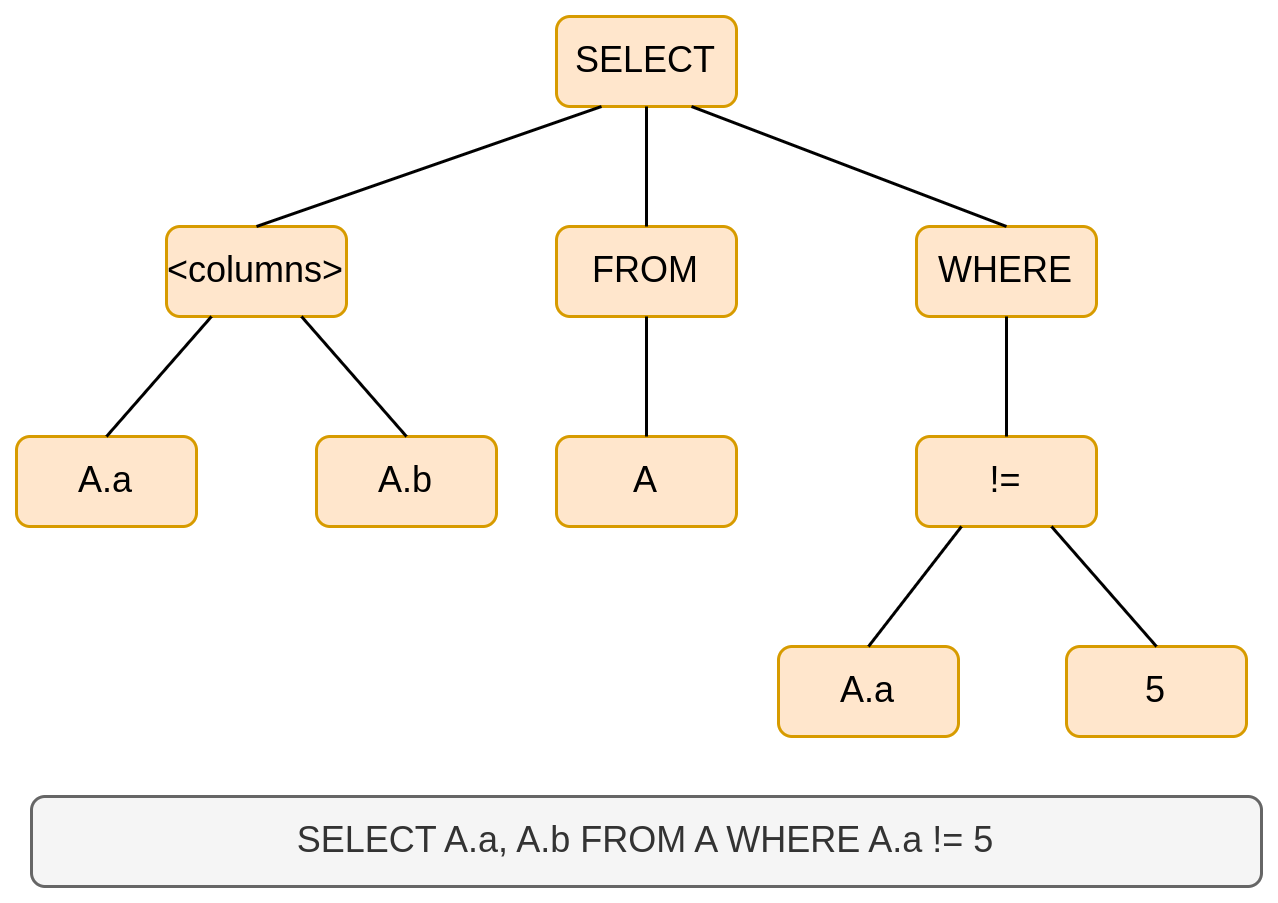
\includegraphics[width=0.6\linewidth]{images/ast_example.png}
  \caption{Drzewo AST dla przykładowego zapytania SQL}
  \label{fig:ast-example}
\end{figure}

Wspomnianym problemem z wykorzystaniem AST jest to, że przetłumaczone z wykorzystaniem biblioteki \code{sqlglot} zapytania, chociaż pod względem semantycznym pozostają bez zmian, to modyfikacji ulega ich formatowanie - następuje zmiana sposobu nawiasowania, czy też stawiania białych znaków. Przekonwertowane w ten sposób zapytania odbiegają więc istotnie od oryginalnych i porównywanie takiego zbioru z oryginalnym \code{Spider} mogło by być kwestionowane. Ponadto wiele algorytmów opiera się na specyficznym dla zbioru \code{Spider} formacie zapytań i jego modyfikacja doprowadziła by do problemów z uruchomieniem wielu modeli. Z przytoczonych powodów porzucono to podejście.

W celu dokonania modyfikacji schematu w zapytaniach, bez niepotrzebnego wpływania na ich strukturę, zdecydowano się ostatecznie zrobić to na niższym poziomie. W tym celu opracowano algorytm, który najpierw dokonuje tokenizacji zapytań, a następnie analizuje wszystkie tokeny po kolei i jeżeli trafi na nazwę kolumny lub tabeli to dokonuję podmiany na nową nazwę. Aby sprawdzić, czy dany token jest nazwą kolumny lub tabeli dokonywano parsowania zapytania do AST, następnie zmieniano dany token na inny i ponownie parsowano zapytanie do AST. Porównując ze sobą te dwa drzewa AST można było ustalić, czy zmodyfikowanym tokenem była nazwa tabeli, nazw kolumny, czy żadne z powyższych.

W celu przetłumaczenia nazwy kolumny należało dodatkowo ustalić, do jakiej tabeli ona należy. Aby to zrobić konieczne było rozpatrzenie trzech możliwych przypadków:

\begin{enumerate}
    \item Nazwa kolumny poprzedzona nazwą tabeli (\sql{SELECT order.id FROM order})
    \item Nazwa kolumny poprzedzona aliasem (\sql{SELECT T1.id FROM order as T1})
    \item Nazwa kolumny bez tabeli (\sql{SELECT id FROM order})
\end{enumerate}

Pierwszy scenariusz jest najprostszy, ponieważ nazwa tabeli jest jawnie podana i nie ma co do niej wątpliwości. Drugi przypadek jest bardziej skomplikowany ponieważ zamiast istniejącej nazwy tabeli wykorzystany został stworzony alias, więc wcześniej trzeba wydobyć z zapytania wszystkie aliasowania. Trzeci przypadek jest również trudny, ponieważ kolumna należy do jednej z wykorzystanych w zapytaniu tabel, więc trzeba wiedzieć dodatkowo jakie tabele są dostępne. Dla tych dwóch przypadków sytuację dodatkowo komplikuję fakt, że zapytania mogą być swobodnie zagnieżdżanie i łączone szeregowo za pomocą operatorów zbiorowych, co skutkuje tym, że w obrębie pojedynczego zapytania pojawiają się zakresy w których dostępne są różne tabele i różne aliasowania.

Aby poradzić sobie z ustaleniem przynależności kolumn do tabel w skomplikowanych zapytaniach postanowiono więc dokonywać rekurencyjnego rozbijania składających się na nie tokenów, przekazując przy tym kontekst mówiący o obowiązującym aliasowaniu z zapytań nadrzędnych do podrzędnych. Zostało to zilustrowane na rysunkach 
\ref{fig:query-decomposition-serial} oraz \ref{fig:query-decomposition-nested}. Przedstawiają one odpowiednio dekompozycję zapytania zawierającego operator zbiorowy oraz dekompozycję zapytania z zagnieżdżeniem. W tym drugim przypadku miejsce zapytania podrzędnego jest zastępowane poprzez fragment \sql{SELECT 1}, aby zapewnić strukturalną poprawność obu wynikowych zapytań. W wyniku tego procesu otrzymywany jest zbiór elementarnych zapytań wraz z obowiązującymi wewnątrz nich kontekstami, co pozwala na łatwą modyfikację tokenów odpowiadających za nazwy tabel i kolumn. Jako, że pierwotnym źródłem tych tokenów jego wejściowe, skomplikowane zapytanie to również ono jest tłumaczone - niejako jako efekt uboczny, lecz jest to celowym zamierzeniem.

% Podczas tego procesu kontekst z zapytań nadrzędnych, jest przekazywany do zapytań podrzędnych, aby utrzymywać przez cały czas informację o dostępnych w danej części zapytania aliasowaniach.

\begin{figure}[ht!]
  \centering
  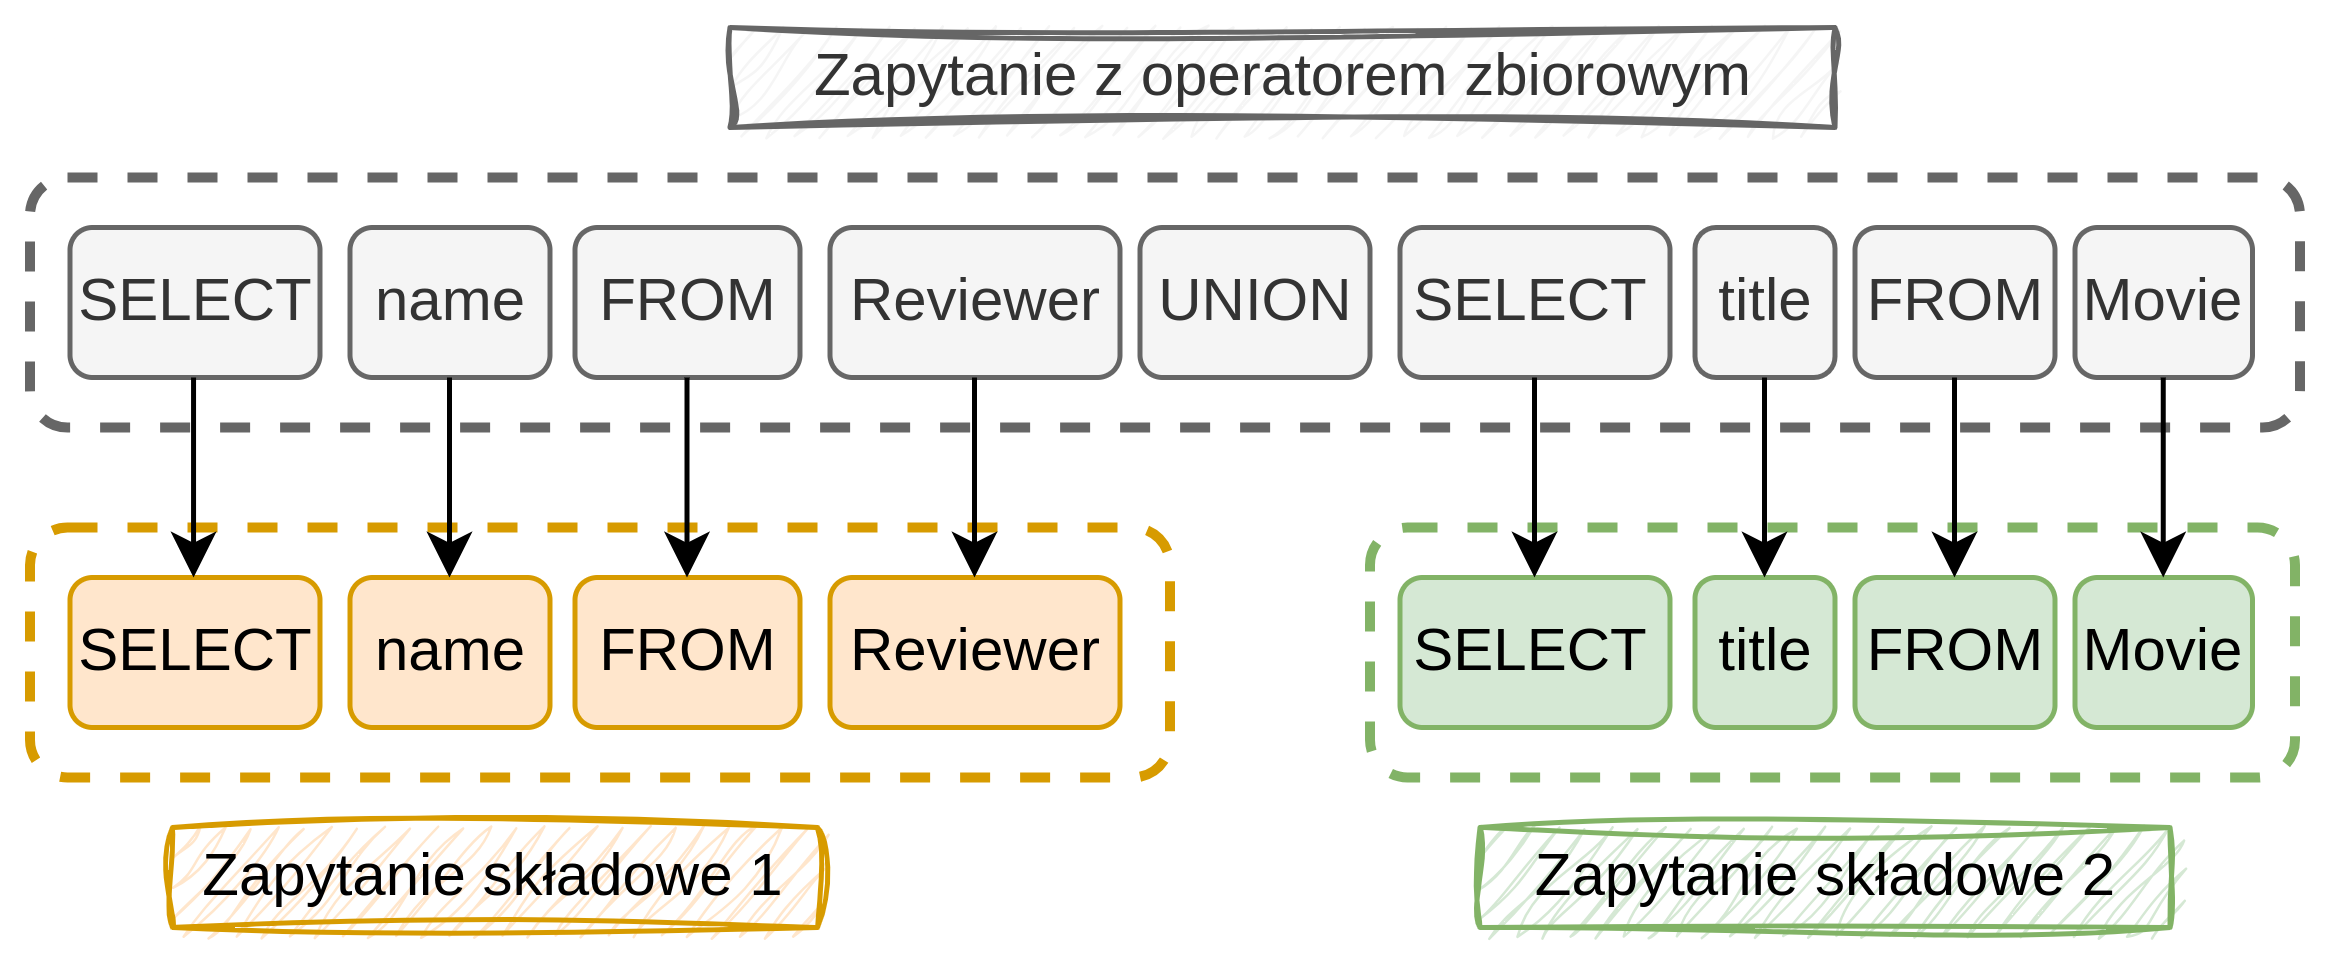
\includegraphics[width=1.0\linewidth]{images/query_decomposition_serial.png}
  \caption{Metoda dekomponowania zapytań z operatorami zbiorowymi}
  \label{fig:query-decomposition-serial}
\end{figure}

\begin{figure}[ht!]
  \centering
  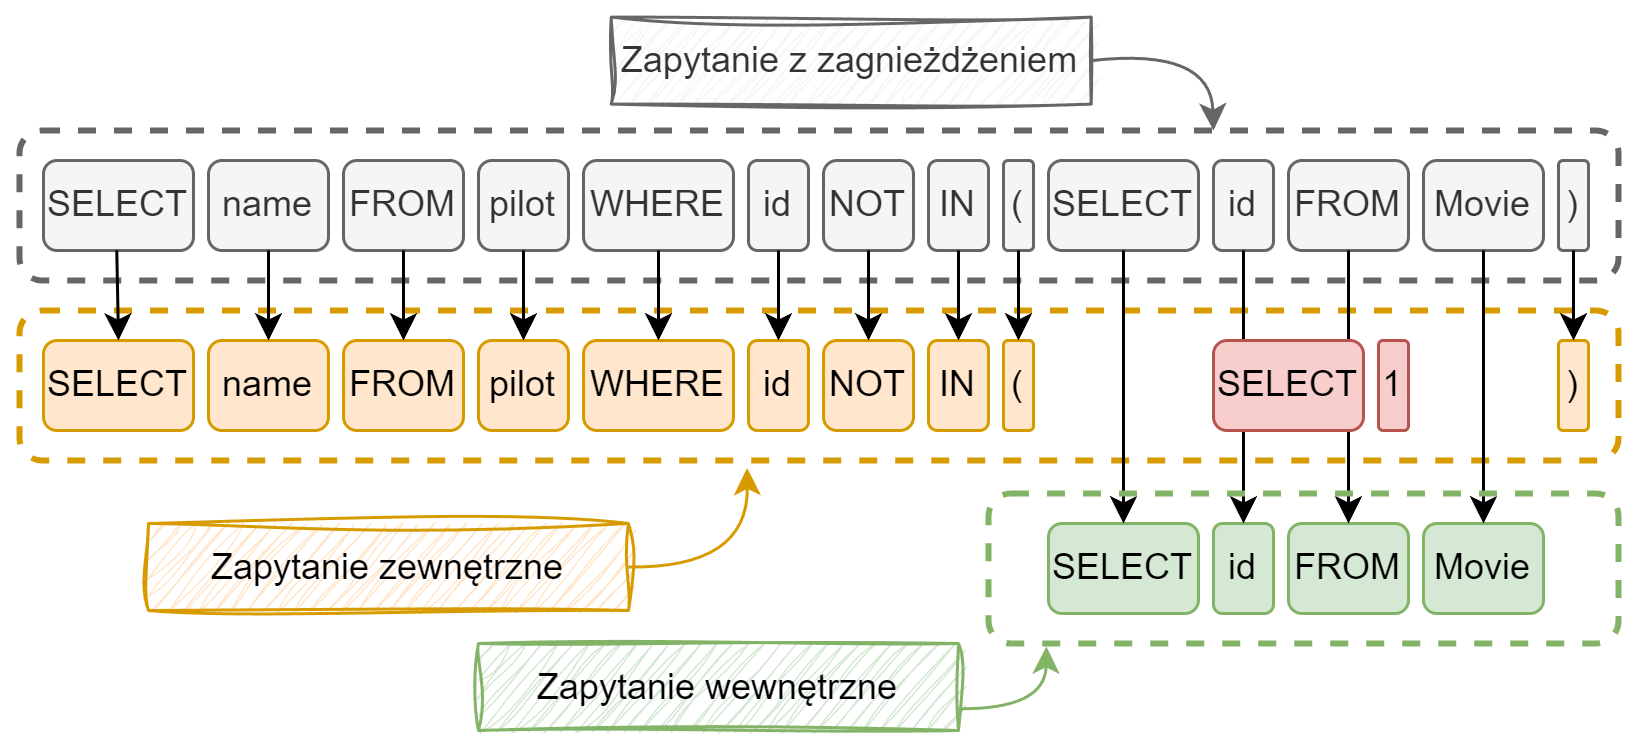
\includegraphics[width=1.0\linewidth]{images/query_decomposition_nested.png}
  \caption{Metoda dekomponowania zapytań zagnieżdżonych}
  \label{fig:query-decomposition-nested}
\end{figure}



\subsection{Dodawanie informacji redundantnych}
Jak zostało wcześniej wspomniane i zademonstrowane na listingach, z źródłowych danych wykorzystywanych do generowania finalnego zbioru zostały usunięte informacje redundantne, aby umożliwić łatwiejsze operowanie nimi. W procesie ostatecznej syntezy należy jednak te informacje ponownie odtworzyć, aby stworzony zbiór w żaden sposób nie odbiegał formatem od oryginalnego.

\subsubsection{Tokenizacja zapytań SQL}
Jednym z elementów, które trzeba dodać do wynikowego zbioru są zapytania SQL podzielone na tokeny. Występują one wewnątrz próbek pod kluczem \code{question\_toks}. Okazuję się, że duża część istniejących rozwiązań nie wykorzystuje tej informacji, ponieważ tokenizacji można dokonać na różne sposoby i wiele modeli wykonuję ją samemu, wybierając sposób dla siebie najkorzystniejszy. Nie mniej jednak pierwsze modele, jak i zapewne część nowszych, korzysta z dostarczonego w ramach zbioru sposobu tokenizacji, więc jeden z nich został wybrany i zaimplementowany.

Oryginalny sposób tokenizacji zapytań wydaje się dość nienaturalny, ponieważ poza klasycznym podziałem na słowa dokonywana jest również zamiana cudzysłowów rozpoczynających na tokeny \code{``} oraz cudzysłów zamykających na tokeny \code{''}. Okazuję się, że jest to sposób tokenizacji promowany przez bibliotekę \code{nltk}, która prawdopodobnie została używa przez autorów. Wyjaśnieniem dla takiego zachowania jest to, że cudzysłowy rozpoczynające i zamykające pełnią różne funkcję, więc może warto zachować tą informację poprzez zamianę ich na osobne tokeny. Obecne modele, w szczególności te oparte o architekturę transformerów, nie powinny mieć jednak najmniejszych problemów z nauką związku pomiędzy cudzysłowami bez tej dodatkowej informacji, więc postanowiono zastosować prostszy sposób tokenizacji - co zrobili również autorzy wcześniejszych tłumaczeń.

\subsubsection{Tokenizacja zapytań SQL bez wartości}


Opracowany algorytm jest niemal całkowicie zbieżny z wykorzystanym w oryginalnym zbiorze \code{Spider} sposobem tokenizacji. Aby to zweryfikować za jego pomocą dokonano tokenizacji oryginalnych zapytań i sprawdzano, czy wyniki pokrywają się z oryginalnymi tokenami. Okazuję się, że różnice występują jedynie w 18 przypadkach spośród prawie dziesięciu tysięcy. Sposób tokenizacji tych kilkunastu zapytań jednak znacznie odbiega od całej reszty i przypuszcza się, że stanowią one niedopracowanie i niespójność oryginalnego zbioru.

Stworzony algorytm w dużym mierze opiera się na bibliotece \code{sqlparse}, która pierwotnie dokonuje tokenizacji. Następnie jednak część tokenów jest rozbijana na mniejsze, lub agregowana w większe, by dopasować się do oryginalnego sposobu tokenizacji. Przykładem rozbijania, jest rozłożenie operatorów porównywania, takich jak \sql{!=}, \sql{>=}, \sql{<=} na pojedyncze znaki. Agregowane są natomiast

\subsection{Parsowanie zapytań SQL}

\subsubsection{Tokenizacja pytań}

\section{Wykonywanie tłumaczenia}

\section{Podsumowanie stworzonych zbiorów}
